As defined in section \ref{sec:ssa_design}, the goal of the Server Side Application is to serve the CSA with the solution to FTP requests. Its corresponding API is publicly accessible \footnote{The developed API has the following URL: \url{https://safe-plateau-51528.herokuapp.com/documentation}} and is used by the CSA to communicate with the CSA. Upon establishing a connection, the Uniform Resource Identifier (URI) of the FTP request is used to identify a particular resource corresponding to the the set of user selected input arguments. This is discussed with more detail in subsection \ref{sec:api_protocol}.
%The Server Side Application is built using Python and a Python framework denoted Django, which facilitates the construction of servers and APIs. Django enables the creation of routes for the application, and each of these is connected to a particular set of instructions. It is also possible to define a pattern each route, enabling the setting of user selected input. \todo{shit paragraph}



%This data is used as input to a python class called \textit{Resource}. Upon creating the Resource object, the user defined request is validated. In case there is an error in the data, for example a past date, or an invalid airport/city, the proccess does not continue, and Django responds with an error. On the other hand, if the validation is succesfull, the Resource object creates a second class object, called \textit{Request} object. There are 3 types of request objects: the \textit{single}, \textit{round} and \textit{multicity} trip. These objects are not to be confused with the respective single/round flight. While a flight corresponds to a single instance connecting two locations in a particular date, a single/round flight may have an extended start period, in which case there are several flights which may constitute a solution to a user request.

To construct a solution to a given request, it is necessary to sequentially execute a particular set of steps, denoted as the \textit{main cycle} of the SSA, which can be summarized as follows: 
%Every Request class has a particular set of functions which are executed each time the class is instantiated. This set of instructions are called the \textit{main} cycle of each request object, and correspond to the:

\begin{enumerate}%[noitemsep,topsep=0pt,parsep=0pt,partopsep=0pt]
  \item generate the list of necessary flights;
  \item request flight data from third-party API;
  \item construct the weight matrix for the objective functions;
  \item execute the optimization algorithms;
  \item construct a solution to the request.
\end{enumerate}

Each step of the \textit{main cycle} is executed by a particular set of functions. Steps number 1), 3) and 5) are managed by a predefined python class, which implements the logic associated to each FTP request. This class is also responsible for the communication with the DMS and OS, which execute steps number 2) and 4), respectively. It should be noted that the execution of the optimization step (iv) is only required for multi-city flight requests, since, for the single-flight and round trip, determining the best solution is a trivial task.

%From this main cycle, steps i), iii) and v) are handled internally by python defined class objects, while steps ii) and iv) are managed by the Data Management and Optimization systems, respectively. 


The implemented SSA dataflow is illustrated in figure \ref{fig:api_structure}. By using the utilities offered by django, the SSA implements a server with a single endpoint, where the requests from the CSA are received. These requests must be validated, in order to discard meaningless queries. This validation occurs immediately after receiving the request. It uses regular expressions to parse the request, followed by an analysis of the input arguments, according to the rules defined in table \ref{table:api_symbols} of the following subsection. After the validation, the resources are translated into a FTP request, and, in particular, to a python object that executes the previously described \textit{main cycle}.


%Figure \ref{fig:api_structure} illustrates the structure of the Client Side Application. This application is activated each time a request is received, which activates  the instantiation of a \textit{Resource} object, responsible for the validation of the request. After a successfull validation, the Resource object instantiates a \textit{Request} object, which executes the \textit{main cycle} of the solution construction procedure, by first calling the Data Management System to collect the necessary set of flights, following this with the execution of a series of optimization algorithms, to produce a stream of responses which can be served to respond to the request.

\begin{figure}[htpb]
  \centering
  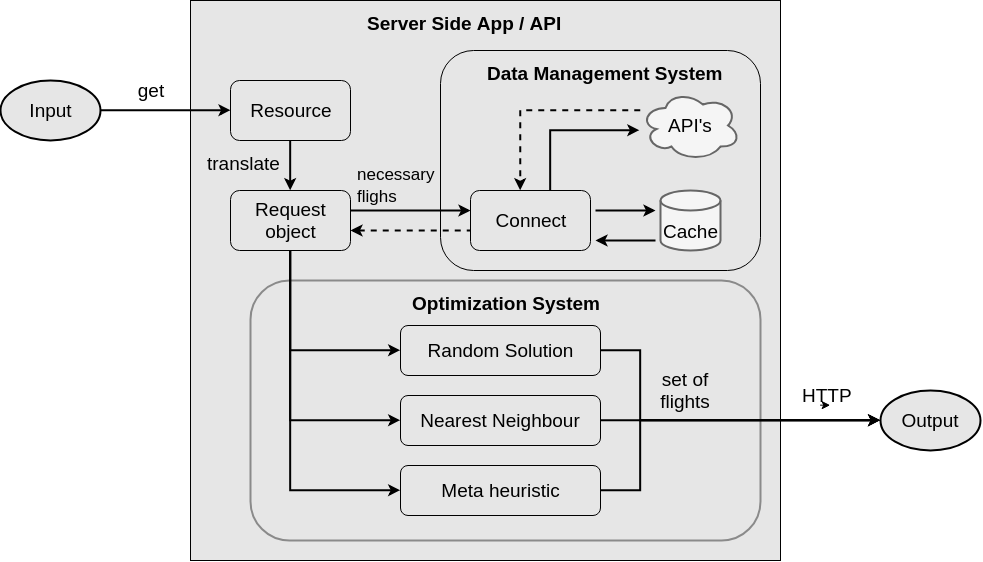
\includegraphics[width=\textwidth]{./Figures/system_implementation/api.png}
  \caption{Server Side Application dataflow}
  \label{fig:api_structure}  
\end{figure}